\section{Auswertung}
\label{sec:Auswertung}

\subsection{Spektrum des \textsuperscript{137}Cs-Strahlers}

Das aufgenommene Spektrum des \textsuperscript{137}Cs-Strahlers ist in Abbildung
\ref{fig:verlauf} dargestellt.

\begin{figure}[H]
  \centering
  \includegraphics{verlauf.pdf}
  \caption{Aufgenommenes Spektrum des \textsuperscript{137}Cs-Strahlers.}
  \label{fig:verlauf}
\end{figure}

Eindeutig zu erkennen ist das Compton-Kontinuum im Bereich kleiner Channel (Energien).
Im Bereich um Channel $90$ ist dann die Compton-Kante zu finden. In diesem Bereich
fällt die Anzahl an Counts noch einmal eindeutig ab. Der eigentliche Peak der $\gamma$-Strahlung der Caesium-Quelle
ist dann in einem Bereich um Channel 127 zu erkennen. Dieser hat eine gewisse Breite,
weshalb im Folgenden die Zählraten durch Integration über eben diesen Bereich im
entsprechenden Spektrum ermittelt werden.

\subsection{Abschwächung des ersten Würfels}
Die gemessenen Counts $N$ des ersten Würfels, sowie die daraus resultierenden Zählraten  $I_{0,\mathrm{i}}$ bei einer Messung
über $\SI{20}{\second}$ sind in Tabelle \ref{tab:w1} dargestellt.

\begin{table}[H]
  \centering
  \caption{Zählrate in Abhängigkeit der Projektion bei einer Messdauer von $\SI{20}{\second}$ }
  \label{tab:w1}
  \begin{tabular}{c c c}
    \toprule
    Projektion & $N$ & $I_{0,\mathrm{i}}$   \\
    \midrule
        $I_1$    & $\SI{16161(152)}{}$ & $\SI{808.05(760)}{}$    \\
        $I_2$    & $\SI{16165(151)}{}$ & $\SI{808.25(755)}{}$    \\
        $I_3$    & $\SI{16218(151)}{}$ & $\SI{810.90(755)}{}$    \\
        $I_4$    & $\SI{15596(151)}{}$ & $\SI{779.80(755)}{}$    \\
        $I_5$    & $\SI{15662(151)}{}$ & $\SI{783.10(755)}{}$    \\
        $I_6$    & $\SI{15899(152)}{}$ & $\SI{794.95(760)}{}$    \\
        $I_7$    & $\SI{15997(153)}{}$ & $\SI{799.85(765)}{}$    \\
        $I_8$    & $\SI{16187(152)}{}$ & $\SI{809.35(760)}{}$    \\
        $I_9$    & $\SI{16213(153)}{}$ & $\SI{810.65(765)}{}$    \\
        $I_{10}$ & $\SI{15509(151)}{}$ & $\SI{775.45(755)}{}$   \\
        $I_{11}$ & $\SI{15725(151)}{}$ & $\SI{786.25(755)}{}$    \\
        $I_{12}$ & $\SI{15605(152)}{}$ & $\SI{780.25(760)}{}$    \\
    \bottomrule
  \end{tabular}
\end{table}

Die $I_{0,\mathrm{i}}$ sind für die weiteren Berechnungen die Ausgangszählraten.




\subsection{Abschwächungskoeffizienten des vierten Würfels}
Die Abschwächungskoeffizienten der einzelenen Materialien werden mit Gleichung (3) bestimmt. Die Dicke
der Elementarwürfel beträgt dabei $d=\SI{1}{\centi\meter}$. In Tabelle (?) werden die gemessenen Zählraten und
die daraus berechneten Abschwächungskoeffizienten dargestellt.

\begin{table}[H]
  \centering
  \caption{Zählrate in Abhängigkeit der Projektion bei einer Messdauer von $\SI{300}{\second}$ und und Abschwächungskoeffizienten }
  \label{tab:Parameter}
  \begin{tabular}{c c c | c c}
    \toprule
    Projektion & $N$ & Fehler & $\mu$ & Fehler   \\
    \midrule
        $I_1$    & 16161 & 152 & &    \\
        $I_2$    & 16165 & 151 & &    \\
        $I_3$    & 16218 & 151 & &    \\
        $I_4$    & 15596 & 151 & &    \\
        $I_5$    & 15662 & 151 & &    \\
        $I_6$    & 15899 & 152 & &    \\
        $I_7$    & 15997 & 153 & &    \\
        $I_8$    & 16187 & 152 & &    \\
        $I_9$    & 16213 & 153 & &    \\
        $I_{10}$ & 15509 & 151 & &   \\
        $I_{11}$ & 15725 & 151 & &    \\
        $I_{12}$ & 15605 & 152 & &    \\
    \bottomrule
  \end{tabular}
\end{table}


\begin{figure}
  \centering
  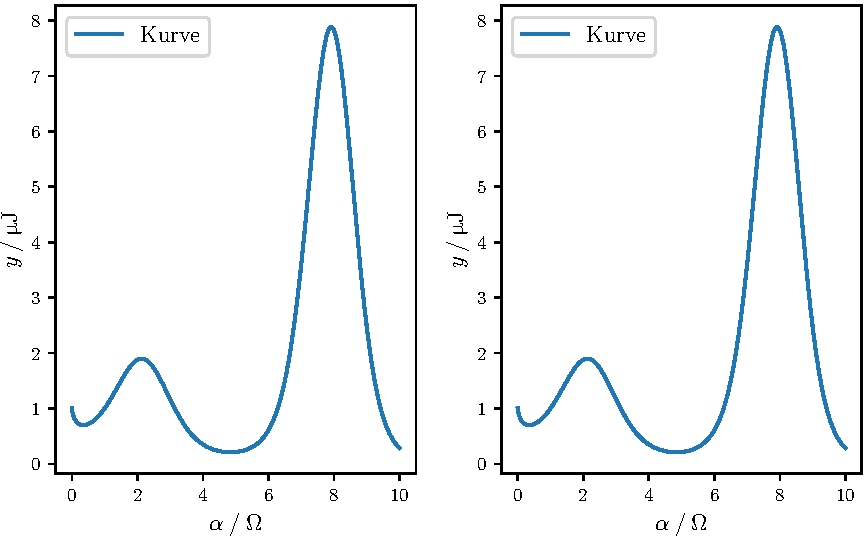
\includegraphics{plot.pdf}
  \caption{Plot.}
  \label{fig:plot}
\end{figure}
